\chapter{Introduction}\label{ch1:Intro}

%Try to describe the mechanical response of materials from first principles is an intelectual exercise that I found to be interesting enough to dedicate 2 years of my time and maybe more.

% About this thesis

I found it very interesting to explore how to describe material's mechanical response from first principles, and I devoted two years to this research, with the possibility of extending it further.
Despite the financial constraints and significant computational resources required to solve quantum mechanical systems, we have implemented a feasible computational methodology to investigate the correlation between molecular geometrical structure and mechanical response.
In addition, the computational methodology is based on a numeric protocol that replicates the polymeric network of PNIPAM microgels, which are a size-tunable hydrogel.

From a brief literature review has revealed the extensive range of applications for hydrogels in various fields.
And a thorough review of the existing literature has revealed a lack of consensus on the precise ``origin'' of the mechanical response exhibited by hydrogels.
In this regard, the key objective of the thesis is to explore a computational methodology for identifying parameters that can represent the main properties of the polymeric network. 
These parameters can then be coupled into a constitutive relations to predict the mechanical response of a simplified polymeric network.
To that end, we have established the following specific objectives:
\begin{itemize}
    \item Replicate the numeric protocol.
    \item Adapt the protocol to create a more general network.
    \item Apply shear deformation to the network.
    \item Characterize the network before and after shear.
    \item Analyze the strain-stress curves of the material under different shear conditions and different network parameters.
\end{itemize}
We expect that the analysis will assist us in selecting a parameter or a combination of parameters to couple them into a constitutive equation.
It is important to clarify that the definition of the constitutive equation or the mathematical procedure/proposal are not within the scope of this thesis. 
The objective is to identify a relation between network characteristics and mechanical response of the network.

In the following section, we will explore the applications of hydrogels identified during the literature review. 
We will also introduce the main characteristics of the mechanical response in general terms.
The subsequent theoretical framework chapter begins by explaining how to quantify the properties of the material and how to apply numerical simulations to analyze the system.
Finally, we closed with the analysis of the numerical solutions chapter and the conclusion of this work.

\section{About Hydrogels}

While the numerical protocol was initially developed for a specific polymeric network, we modified it to represent a more simplified case that resembles a broader group of polymeric networks.
These polymeric networks are collectively referred to as hydrogels.
Hydrogels are composed primarily of hydrophilic monomers, which are biocompatible, making them suitable for medical applications.
In general terms, hydrogels exhibit visco-elastic and visco-plastic mechanical responses.
The material's viscoelasticity response makes it suitable for use in shock absorption, vibration damping, and biological tissue mimicry.
Meanwhile, the viscoplasticity response makes the material suitable for energy dissipation.
First, we will explore various applications of this material.
Then, we will provide a brief introduction to viscoelasticity and viscoplasticity responses.

\subsection{Applications}

The selection of applications is guided by several key factors. 
First, considering the imminent threat that climate change poses to the global environment, investigating environmentally relevant applications is a priority.
Second, to align with the institution's strategic research interests in biomedical applications, we have included examples from this sector.
Finally, I was very interested in seeing applications of smart materials in this sector, based on my academic experience.
Figure~\ref{fig:applications} provides graphical representations of the applications of the hydrogels discussed in this review article \citep{petelinsekToughHydrogelsLoadBearing2024}.
Without further ado, here are some potential applications of this material.

%\paragraph{Environmental applications} 
By modulating the chemical structure, hydrogels can effectively remove a wide range of toxic compounds, such as heavy metals, organic pollutants, pathogens, or nutrients, or environmental parameters.
In the article\citep{cinfrigniniGoldRushDesigning2024} explores an easy-to-make poly(acrylamide-co-acrylic acid) hydrogels as adsorbents for gold recovery from industrial wastewater containing other precious metals.
In this review\citep{randoFunctionalBioBasedPolymeric2024} investigates the emerging topic of stimuli-responsive smart hydrogels, underscoring their potential in both sorption and detection of water pollutants.
On this other review\citep{darbanHydrogelBasedAdsorbentMaterial2022a} explains the synthesis and adsorption mechanicsms in detail with the understanding of the regeneration, recovery, and reuse of hydrogel-based adsorbent materials.
Finally in the article\citep{songSynthesisHydrogelsTheir2022} different synthetic strategies, crosslinking methods and their corresponding limitations and outstanding contributions of applications in the fields of removing environmental pollutants are reviewed to further provide a prospective view of their applications in water resources sustainability.

%\paragraph{Medical applications} 
Hydrogels, have garnered significant attention as versatile materials in biomedical applications due to their high water content, biocompatibility, and tunable properties. 
They mimic natural tissue environments, enhancing cell viability and function.
In the article\citep{wuAdvancementsHydrogelsCorneal2024} they discuss the fundamentals of hydrogels, emphasizing their relevance to corneal tissue engineering, and explore various types of hydrogels, including stimuli-responsive variants.
In the article\citep{kaurHydrogelsPotentialBiomaterial2024} highlight some of the recent interesting applications of bioactive hydrogels in the field of antibacterial wound healing, oral delivery of drugs, cancer immunotherapy, tissue regeneration, and similar potential biomedical aspects.
In the article\citep{thummaIntroductionClassificationApplications2025} presents a thorough investigation of the synthesis and medicinal uses of different naturally occurring and synthetic hydrogels, for cancer therapy, mainly via 3D modeling and printing.

%\paragraph{Smart materials} 
Stimuli responsive hydrogels are emerging as smart materials due to their tunable chemical and physical properties in response to various stimuli like pH, temperature, chemicals, pressure, electrical or light. 
In this review article \citep{bishnoiCellulosebasedSmartMaterials2024}, we have discussed the role and overview of cellulose‐based hydrogels in elements of energy storage systems.
In the article \citep{zhaoIntelligentHydrogelActuators2021} near infrared laser driven intelligent hydrogel actuator systems with a high response rate were prepared via three-dimensional printing and hydrothermal synthesis.
In this review article\citep{shomePhotoresponsiveSmartHydrogels2024}, basic mechanisms responsible for photo-responsiveness in hydrogels along with their potential applications are discussed.
In this review\citep{duttaSmartMaterialsFlexible2024}, they discuss the state-of-the-art applications of hydrogels in flexible electronics, such as energy storage, touch panels, memristor devices, and sensors like temperature, gas, humidity, chemical, strain, and textile sensors, and the latest synthesis methods of hydrogels.

\begin{figure}[ht!]
    \centering
    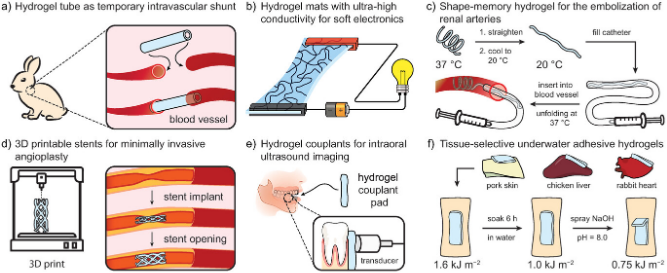
\includegraphics[width=\textwidth]{figs/applications.png}
    \caption{Chosen examples of tough hydrogels applied in the areas of a) tissue engineering, b) soft electronics, c) shape memory materials, d) 3D printing, e) biomedical devices, and f) adhesives. Notably, the majority of the highlighted examples ultimately serve biomedical applications\citep{petelinsekToughHydrogelsLoadBearing2024}.}\label{fig:applications}
\end{figure}


\subsection{Mechanical response}

The origin of the mechanical properties of hydrogels from first principles remains incompletely understood due to the complex multi-scale nature of these materials\citep{senffTemperatureSensitiveMicrogel1999}.
Hydrogels consist of heterogeneous, often disordered polymer networks swollen with water, where molecular interactions (covalent bonds, physical crosslinks, entanglements, and solvent–polymer interactions) collectively determine macroscopic elasticity and viscoelasticity. 
Accurately bridging atomic-scale forces and chemical bond dynamics to bulk mechanical behavior involves coupling nonlinear polymer physics, solvent effects, and dynamic crosslink kinetics. 
Which presents a significant challenge to current theoretical and computational models. 

Viscoelastic materials exhibit a mechanical response that lies between elastic and plastic deformation.
Hydrogels, initially respond elastically to a force and then undergo continuous viscous deformation.
This continuous viscous deformation is known as ``creep''.
Furthermore, when subjected to a constant strain, viscoelastic materials experience ``stress relaxation'', whereby stress decreases over time after the yield point.

When a hydrogel is deformed, the bonds, intermolecular distances, molecular conformation and chain orientation are modified accordingly.
Furthermore, any molecular event resulting in energy dissipation contributes to viscoelasticity, given the direct correlation between viscosity and energy dissipation.
One such factor is the polymer molecular weight, which affects the movement of entangled polymers.
Another factor that promotes molecular mobility is the interconnectivity and cohesion of the network.
These processes enable network flow under an applied force, thereby facilitating viscoelasticity.

Another molecular mechanism that contributes to viscoelasticity is the strength of the crosslinking mechanisms in the network.
In the case of weak crosslink mechanisms, stress relaxation is observed; however, in strongly crosslinked hydrogels, this process is prevented. 
This is due to the fact that weak bonds permit the release of energy and the separation of elements under force, thereby facilitating network relaxation or creep.
Furthermore, weak bonds are capable of responding to force by dissociating and rebinding, which can result in plastic or permanent deformations.
This is in contrast to strong crosslink mechanisms, which prevent the network from flowing and dissipating energy, thereby promoting the material's predominantly elastic properties.
It is widely accepted that permanent cross-links are responsible for the elastic properties of the material, while dynamic cross-links regulate energy dissipation.

Finally, the water content has a significant impact on the viscoelasticity of the hydrogels.
Applying pressure to the hydrogels causes water to flow in or out of the network, resulting in a time-dependent response due to changes in volume. This leads to strand extension and therefore firmness enhancement.
This phenomenon is known as poroelasticity. 
It is important to note that these changes result in viscous dissipation, which in turn impacts the viscoelastic properties\citep{sheikoArchitecturalCodeRubber2019,courbotRoleExtracellularMatrix2025}.


\begin{figure}[ht!]
    \centering
    \centering
    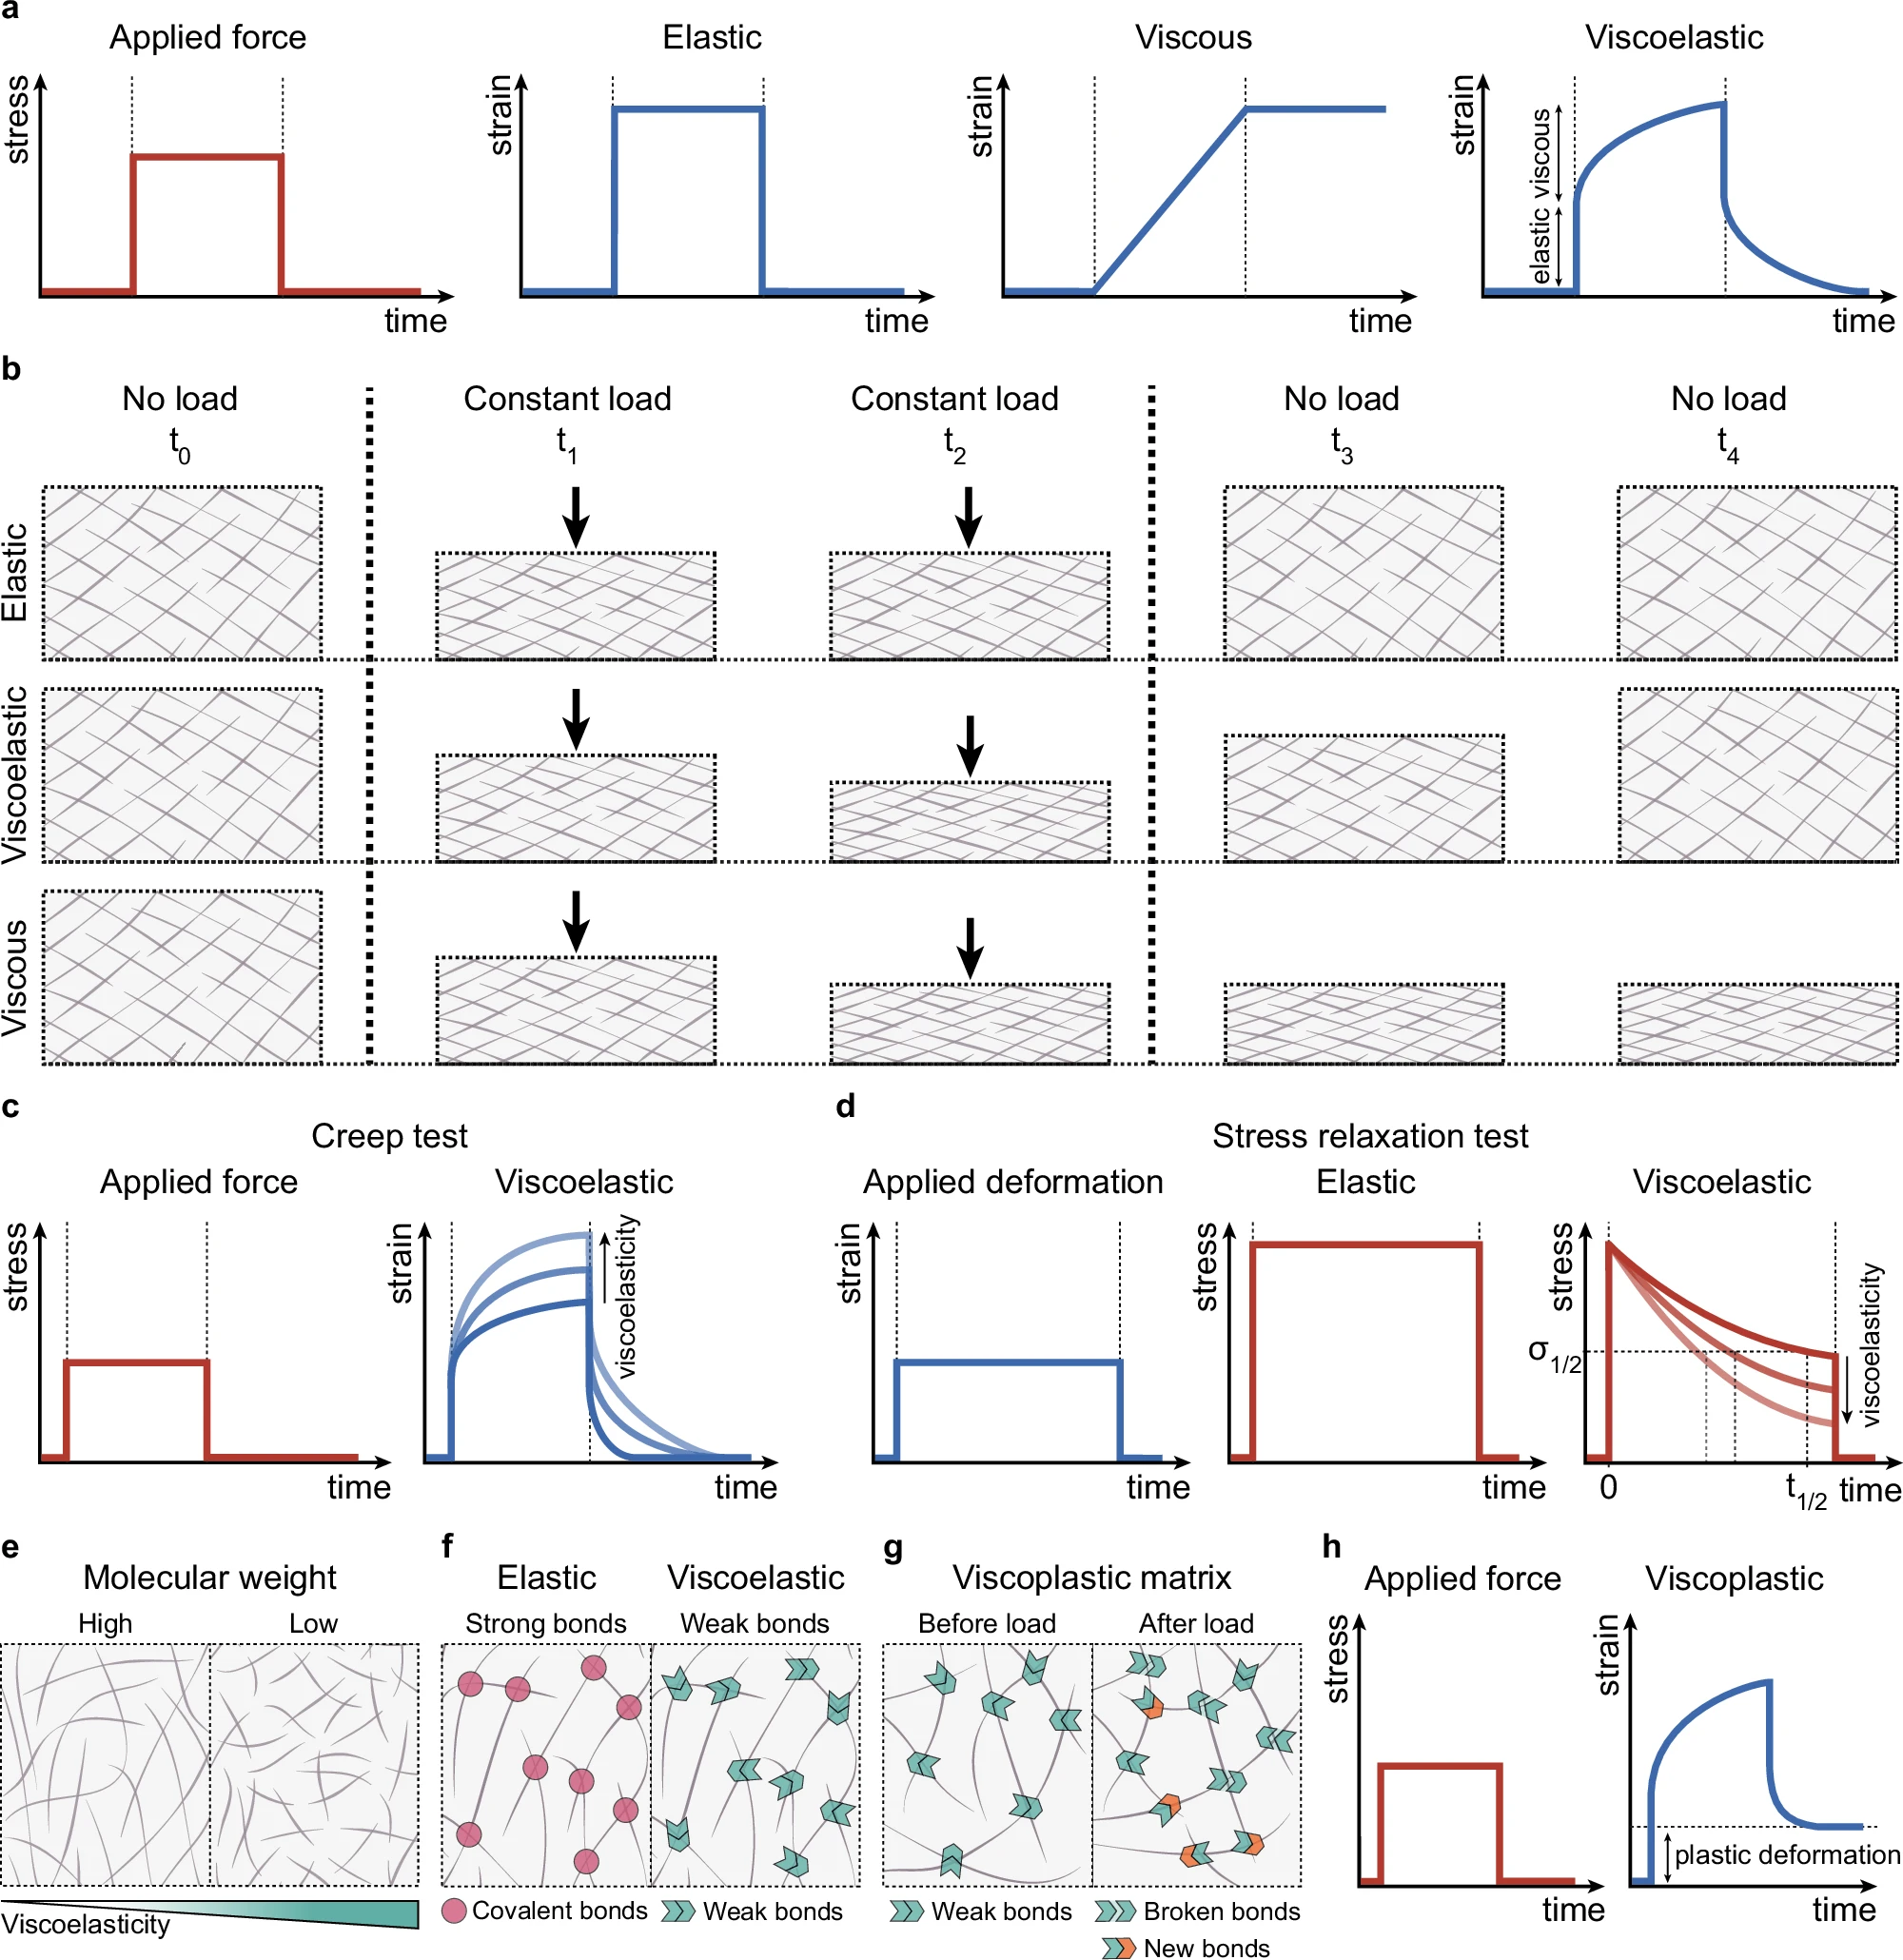
\includegraphics[width=\textwidth]{figs/mechResponse/0.png}
    \caption{Explicar a detalle\citep{courbotRoleExtracellularMatrix2025}}\label{fig:mechresponse0}
\end{figure}

Description of figure\ref{fig:mechresponse0} 
a Under a constant force, purely elastic materials deform instantly and maintain that deformation until the load is removed, at which point they immediately return to their original shape. Different from elastic materials, purely viscous materials undergo continuous deformation. Viscoelastic materials display an initial immediate response to force (elastic component) followed by an increase in the deformation over time (viscous component). Stress and strain colours are red and blue, respectively. b Under a constant force (black arrows), the deformation of a purely elastic matrix is time-independent: the matrix immediately deforms and returns to its initial shape when the force is applied and removed, respectively (top). Contrary to elastic matrices, viscoelastic matrices response changes with time: under a constant load, the deformation increases over time and they do not immediately return to their original shape once the load is removed (middle). Purely viscous matrices will continuously deform due to the force, and retain their deformed shape after the force is removed (bottom). c Creep test showing the deformation of a viscoelastic material in response to a constant force. The more  viscoelastic the material is, the more it deforms over time under the load. d A stress relaxation test shows the evolution of the stress in the material in response to constant deformation. Purely elastic materials experience constant stress. In a deformed viscoelastic material, the stress decreases over time. The stress relaxation half-time (t1/2) is defined as the time needed for the stress to reach half its initial value. The more viscoelastic material is, the faster the stress decreases and, therefore, the lower t1/2 is. e Decreasing the molecular weight of the ECM components decreases the network connectivity and, therefore, increases ECM viscoelasticity, as it favours energy dissipation and fibre movements. f Purely elastic materials are typically crosslinked by covalent bonds (left), while viscoelastic materials usually contain weaker crosslinks such as ionic bonds (right) or physical entanglements that favour stress relaxation. g In viscoplastic materials, permanent deformations remain after the load is removed due to the breaking of bonds and the formation of new bonds. h During a creep test, viscoplastic materials do not return to their original shape and retain permanent deformations\citep{courbotRoleExtracellularMatrix2025}.



